\documentclass{article}

\usepackage{a4}
\usepackage{amsmath}
\usepackage{amssymb}
\usepackage{ctex}
\usepackage{booktabs}
\usepackage{graphicx}
\usepackage{subfigure}
\usepackage{subcaption}
\usepackage{float}
\usepackage{hyperref}
\usepackage{xurl}
\usepackage{enumitem}
\usepackage{array}
\usepackage{longtable}
\usepackage{multirow}
\usepackage{fvextra}

\hypersetup{colorlinks=true,linkcolor=black,urlcolor=blue,citecolor=black}
\setlist[itemize]{nosep,leftmargin=1.8em}
\setlist[enumerate]{nosep,leftmargin=1.8em}
\captionsetup{font=small}
\RecustomVerbatimEnvironment{verbatim}{Verbatim}{
  breaklines=true,
  breakanywhere=true,
  fontsize=\small
}

\title{计算机组成原理 \\ 实验2 数据运算：定点乘法优化与加速}
\author{鲁昕宁 2414015}
\date{\today}

\begin{document}

\maketitle
\begin{center}
    \url{https://github.com/SidneyLu/Computer-Organization-and-Design-NKU-CS/tree/master/lab2}
\end{center}

\newpage

\section{实验目标}
参考实验指导手册第二次的乘法器实验，完成对乘法器的改进：

\section{实验原理}
\subsection{基数为2的 Booth 算法}
给定两个n bit乘数A、B，积为C
A为被乘数，B为乘数，变量i用于标记B中的位数,
Qn表示B的最低位，同时将一个额外的Qn+1添加至B的最后一位
初始化C=0，Qn+1=0，同时将i变量赋值为n.
每次读取最低两位QnQn+1
\begin{itemize}
    \item 10: C = C-A
    \item 01: C = C+A
    \item 00: C不变
    \item 11: C不变
\end{itemize}
将\{C, B, Qn+1\}拼接的结果算术右移一位，保留C的符号位

i = i - 1

while i!=0 repeat
\subsection{Wallace 树}
注意到全加器输入为\{cin, a, b\}，输出为\{cout, sum\}, 不妨用这一特性将3个n位数的相加转换成两个n+1位数的相加，由此在乘法计算中把求和步骤归约。
华莱士树就是利用这一特性把CSF进位保存加法器按层次组织起来的结构。

参考乘法的竖式计算，A和B逐位相乘。应用前文所述的基数为2的 Booth 算法时，可按相邻两位窗口 \(\{b_i,b_{i-1}\}\) 生成多个“部分积”，为了计算最终结果，我们要将部分积求和，对于每一位，使用华莱士树的归约，
例如垂直方向上有八个部分积，这一位就可以按照
\begin{verbatim}
(3，3，2)->(2, 2, 2)
(3, 3)->(2, 2)
(3,1)->(2,1)
(3)->(2)
(2)->(1)
\end{verbatim}
的流程用华莱士树归约.


\section{实验过程}
\subsection{模块设计}
\begin{enumerate}
  \item \textbf{第一层：radix-2 Booth 编码}
    \begin{itemize}
      \item 编码窗口数量：32 位乘数采用重叠的 2 位窗口 \(\{b_i,b_{i-1}\}\)，共产生 32 个 Booth 判决
      \item 输入：乘数扩展为 \(\{B_{31},B_{30},\dots,B_0,B_{-1}\}\)，其中 \(B_{-1}=0\)
      \item 编码规则：\(01 \rightarrow +A\)，\(10 \rightarrow -A\)，\(00/11 \rightarrow 0\)
      \item 输出：32 个符号扩展后的部分积 \(P_{0 \sim 31}\)，第 \(i\) 个部分积左移 \(i\) 位
    \end{itemize}

  \item \textbf{第二层：华莱士树网络}
    \begin{itemize}
      \item 输入：第一层生成的 32 个部分积
      \item 归约方式：使用 3:2 压缩器逐层归约，源码中的层级为 \(32 \rightarrow 22 \rightarrow 15 \rightarrow 10 \rightarrow 7 \rightarrow 5 \rightarrow 4 \rightarrow 3 \rightarrow 2\)
      \item 输出：两路 68 位加数 \(S\) 和 \(C\)
    \end{itemize}

  \item \textbf{第三层：最终加法器}
    \begin{itemize}
      \item 加法器位宽：68 位
      \item 输入：第二层输出的两路加数 \(S\) 和 \(C\)
      \item 输出：先得到 68 位求和结果，再取其低 64 位作为最终乘积
    \end{itemize}
\end{enumerate}

\begin{figure}
  \centering
  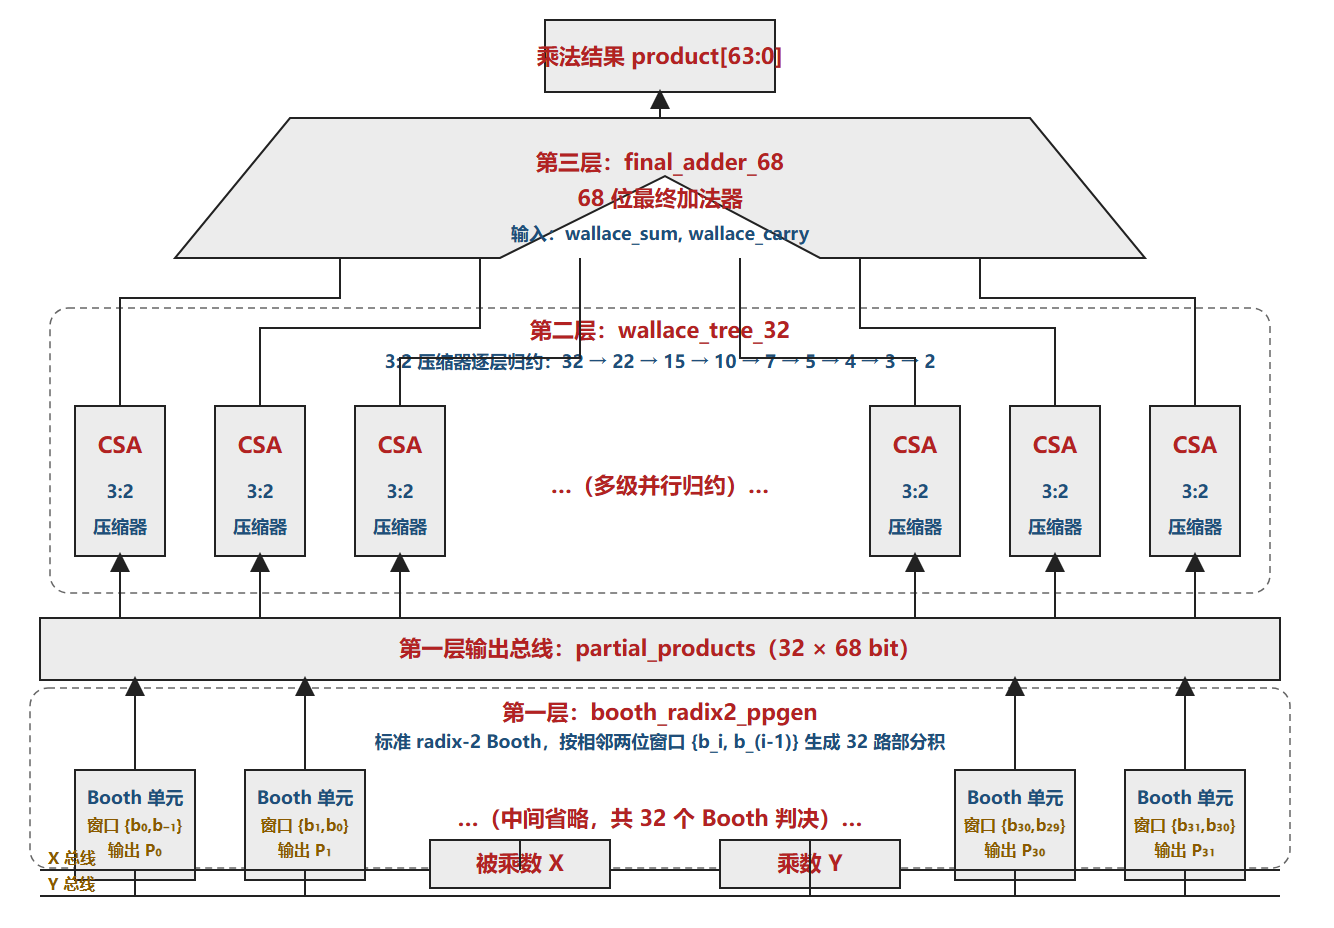
\includegraphics[width=0.8\textwidth]{module.png}
\end{figure}

\newpage
\subsection{源码}
Verilog 源码位于 \verb|lab2/lab2.srcs|，关键片段如下。
\begin{verbatim}
  module booth_radix2_ppgen(
    input  [31:0] mult_op1,
    input  [31:0] mult_op2,
    output [2175:0] partial_products
);

    wire signed [67:0] multiplicand_ext;
    wire [32:0]        booth_bits;

    assign multiplicand_ext = {{36{mult_op1[31]}}, mult_op1};
    assign booth_bits       = {mult_op2, 1'b0};

    function signed [67:0] booth_select;
        input [1:0]         booth_code;
        input signed [67:0] multiplicand;
        reg   signed [67:0] booth_value;
        begin
            case (booth_code)
                2'b01: booth_value = multiplicand;
                2'b10: booth_value = -multiplicand;
                default: booth_value = 68'd0;
            endcase
            booth_select = booth_value;
        end
    endfunction

    genvar g0;
    generate
        for (g0 = 0; g0 < 32; g0 = g0 + 1) begin : GEN_PP
            wire [67:0] pp_value;
            assign pp_value = booth_select(booth_bits[g0 +: 2], 
                                              multiplicand_ext) <<< g0;
            assign partial_products[68*g0 +: 68] = pp_value;
        end
    endgenerate

endmodule

module wallace_tree_32(
    input  [2175:0] partial_products,
    output [67:0]   sum_out,
    output [67:0]   carry_out
);

    function [135:0] csa3;
        input [67:0] a;
        input [67:0] b;
        input [67:0] c;
        reg   [67:0] sum_v;
        reg   [67:0] carry_v;
        begin
            sum_v   = a ^ b ^ c;
            carry_v = ((a & b) | (a & c) | (b & c)) << 1;
            csa3    = {carry_v, sum_v};
        end
    endfunction

    wire [67:0] pp  [0:31];
    wire [67:0] st1 [0:21];
    wire [67:0] st2 [0:14];
    wire [67:0] st3 [0:9];
    wire [67:0] st4 [0:6];
    wire [67:0] st5 [0:4];
    wire [67:0] st6 [0:3];
    wire [67:0] st7 [0:2];
    wire [67:0] st8 [0:1];

    genvar g1;
    generate
        for (g1 = 0; g1 < 32; g1 = g1 + 1) begin : UNPACK_PP
            assign pp[g1] = partial_products[68*g1 +: 68];
        end
    endgenerate

    genvar g2;
    generate
        for (g2 = 0; g2 < 10; g2 = g2 + 1) begin : STAGE1
            wire [135:0] csa_out;
            assign csa_out     = csa3(pp[3*g2], pp[3*g2+1], pp[3*g2+2]);
            assign st1[2*g2]   = csa_out[67:0];
            assign st1[2*g2+1] = csa_out[135:68];
        end
    endgenerate
    assign st1[20] = pp[30];
    assign st1[21] = pp[31];

    genvar g3;
    generate
        for (g3 = 0; g3 < 7; g3 = g3 + 1) begin : STAGE2
            wire [135:0] csa_out;
            assign csa_out     = csa3(st1[3*g3], st1[3*g3+1], st1[3*g3+2]);
            assign st2[2*g3]   = csa_out[67:0];
            assign st2[2*g3+1] = csa_out[135:68];
        end
    endgenerate
    assign st2[14] = st1[21];

    genvar g4;
    generate
        for (g4 = 0; g4 < 5; g4 = g4 + 1) begin : STAGE3
            wire [135:0] csa_out;
            assign csa_out     = csa3(st2[3*g4], st2[3*g4+1], st2[3*g4+2]);
            assign st3[2*g4]   = csa_out[67:0];
            assign st3[2*g4+1] = csa_out[135:68];
        end
    endgenerate

    genvar g5;
    generate
        for (g5 = 0; g5 < 3; g5 = g5 + 1) begin : STAGE4
            wire [135:0] csa_out;
            assign csa_out     = csa3(st3[3*g5], st3[3*g5+1], st3[3*g5+2]);
            assign st4[2*g5]   = csa_out[67:0];
            assign st4[2*g5+1] = csa_out[135:68];
        end
    endgenerate
    assign st4[6] = st3[9];

    genvar g6;
    generate
        for (g6 = 0; g6 < 2; g6 = g6 + 1) begin : STAGE5
            wire [135:0] csa_out;
            assign csa_out     = csa3(st4[3*g6], st4[3*g6+1], st4[3*g6+2]);
            assign st5[2*g6]   = csa_out[67:0];
            assign st5[2*g6+1] = csa_out[135:68];
        end
    endgenerate
    assign st5[4] = st4[6];

    wire [135:0] st6_csa;
    assign st6_csa = csa3(st5[0], st5[1], st5[2]);
    assign st6[0]  = st6_csa[67:0];
    assign st6[1]  = st6_csa[135:68];
    assign st6[2]  = st5[3];
    assign st6[3]  = st5[4];

    wire [135:0] st7_csa;
    assign st7_csa = csa3(st6[0], st6[1], st6[2]);
    assign st7[0]  = st7_csa[67:0];
    assign st7[1]  = st7_csa[135:68];
    assign st7[2]  = st6[3];

    wire [135:0] st8_csa;
    assign st8_csa = csa3(st7[0], st7[1], st7[2]);
    assign st8[0]  = st8_csa[67:0];
    assign st8[1]  = st8_csa[135:68];

    assign sum_out   = st8[0];
    assign carry_out = st8[1];

endmodule

module final_adder_68(
    input  [67:0] addend_a,
    input  [67:0] addend_b,
    output [67:0] sum_out
);

    assign sum_out = addend_a + addend_b;

endmodule

module multiply(
    input         clk,
    input         mult_begin,
    input  [31:0] mult_op1,
    input  [31:0] mult_op2,
    output [63:0] product,
    output        mult_end
);

    wire [2175:0] partial_products;
    wire [67:0]   wallace_sum;
    wire [67:0]   wallace_carry;
    wire [67:0]   product_full;
    wire [63:0]   product_comb;

    reg           mult_begin_d = 1'b0;
    reg [63:0]    product_r    = 64'd0;
    reg           mult_end_r   = 1'b0;

    wire mult_start;
    assign mult_start = mult_begin & ~mult_begin_d;

    booth_radix2_ppgen u_booth_radix2_ppgen (
        .mult_op1        (mult_op1),
        .mult_op2        (mult_op2),
        .partial_products(partial_products)
    );

    wallace_tree_32 u_wallace_tree_32 (
        .partial_products(partial_products),
        .sum_out         (wallace_sum),
        .carry_out       (wallace_carry)
    );

    final_adder_68 u_final_adder_68 (
        .addend_a(wallace_sum),
        .addend_b(wallace_carry),
        .sum_out (product_full)
    );

    assign product_comb = product_full[63:0];

    always @(posedge clk) begin
        mult_begin_d <= mult_begin;
        mult_end_r   <= mult_start;
        if (mult_start) begin
            product_r <= product_comb;
        end
    end

    assign product  = product_r;
    assign mult_end = mult_end_r;

endmodule
\end{verbatim}

\begin{figure}[h!]
  \centering
  
\includegraphics[width=0.8\textwidth]{schematic.png}
\end{figure}

\subsection{仿真验证与分析}
\subsubsection{仿真代码}
\begin{verbatim}
`timescale 1ns / 1ps

module tb;

    reg         clk;
    reg         mult_begin;
    reg  [31:0] mult_op1;
    reg  [31:0] mult_op2;
    wire [63:0] product;
    wire        mult_end;

    localparam integer BASELINE_CYCLES = 32;
    localparam integer MAX_WAIT_CYCLES = 128;

    integer case_id;
    integer pass_count;
    integer fail_count;
    integer total_cycles;
    integer min_cycles;
    integer max_cycles;
    integer i;

    real avg_cycles;
    real saved_cycles;
    real speedup;

    reg signed [31:0] op1_s;
    reg signed [31:0] op2_s;
    reg signed [63:0] expected;

    multiply uut (
        .clk       (clk),
        .mult_begin(mult_begin),
        .mult_op1  (mult_op1),
        .mult_op2  (mult_op2),
        .product   (product),
        .mult_end  (mult_end)
    );

    always #5 clk = ~clk;

    task run_case;
        input [31:0] a;
        input [31:0] b;
        integer cycles;
        integer timeout_flag;
        begin
            case_id = case_id + 1;
            op1_s = a;
            op2_s = b;
            expected = op1_s * op2_s;

            @(negedge clk);
            mult_op1 = a;
            mult_op2 = b;
            mult_begin = 1'b1;

            cycles = 0;
            timeout_flag = 0;

            begin : WAIT_DONE
                while (1'b1) begin
                    @(posedge clk);
                    #1;
                    cycles = cycles + 1;
                    if (mult_end === 1'b1) begin
                        disable WAIT_DONE;
                    end
                    if (cycles >= MAX_WAIT_CYCLES) begin
                        timeout_flag = 1;
                        disable WAIT_DONE;
                    end
                end
            end

            if (timeout_flag) begin
                fail_count = fail_count + 1;
                $display("[CASE %0d] FAIL(timeout): a=%h(%0d), b=%h(%0d), wait_cycles=%0d",
                         case_id, a, $signed(a), b, $signed(b), cycles);
            end else if ($signed(product) !== expected) begin
                fail_count = fail_count + 1;
                $display("[CASE %0d] FAIL(data): a=%h(%0d), b=%h(%0d), got=%h(%0d), exp=%h(%0d), cycles=%0d",
                         case_id, a, $signed(a), b, $signed(b),
                         product, $signed(product), expected, expected, cycles);
            end else begin
                pass_count = pass_count + 1;
                total_cycles = total_cycles + cycles;
                if (cycles < min_cycles) min_cycles = cycles;
                if (cycles > max_cycles) max_cycles = cycles;
                $display("[CASE %0d] PASS: a=%h(%0d), b=%h(%0d), product=%h(%0d), cycles=%0d",
                         case_id, a, $signed(a), b, $signed(b),
                         product, $signed(product), cycles);
            end

            @(negedge clk);
            mult_begin = 1'b0;

            @(posedge clk);
            #1;
            if (mult_end !== 1'b0) begin
                fail_count = fail_count + 1;
                $display("[CASE %0d] FAIL(pulse): mult_end pulse width is not one cycle", case_id);
            end
        end
    endtask

    initial begin
        clk = 1'b0;
        mult_begin = 1'b0;
        mult_op1 = 32'd0;
        mult_op2 = 32'd0;
        case_id = 0;
        pass_count = 0;
        fail_count = 0;
        total_cycles = 0;
        min_cycles = MAX_WAIT_CYCLES;
        max_cycles = 0;
        avg_cycles = 0.0;
        saved_cycles = 0.0;
        speedup = 0.0;

        repeat (3) @(posedge clk);

        run_case(32'h00001111, 32'h00001111);
        run_case(32'h00001111, 32'h00002222);
        run_case(32'h00000002, 32'hffffffff);
        run_case(32'h00000002, 32'h80000000);
        run_case(32'h7fffffff, 32'h7fffffff);
        run_case(32'h80000000, 32'h80000000);
        run_case(32'h80000000, 32'h7fffffff);
        run_case(32'hffff0001, 32'h0000ffff);
        run_case(32'h00000000, 32'hffffffff);

        for (i = 0; i < 100; i = i + 1) begin
            run_case($random, $random);
        end

        if (pass_count > 0) begin
            avg_cycles = (total_cycles * 1.0) / pass_count;
            saved_cycles = BASELINE_CYCLES - avg_cycles;
            speedup = BASELINE_CYCLES / avg_cycles;
        end

        $display("============================================================");
        $display("Summary:");
        $display("  Total cases                 : %0d", case_id);
        $display("  PASS / FAIL                 : %0d / %0d", pass_count, fail_count);
        $display("  Baseline cycles (before)    : %0d", BASELINE_CYCLES);
        if (pass_count > 0) begin
            $display("  Optimized cycles (after)    : min=%0d, max=%0d, avg=%0.2f",
                     min_cycles, max_cycles, avg_cycles);
            $display("  Cycles saved (avg)          : %0.2f", saved_cycles);
            $display("  Speedup (avg)               : %0.2fx", speedup);
        end
        if (fail_count == 0) begin
            $display("  Final result                : ALL PASS");
        end else begin
            $display("  Final result                : HAS FAILURES");
        end
        $display("============================================================");

        $finish;
    end

endmodule
\end{verbatim}

\subsection{波形分析}
仿真脚本已经内置验证乘法结果正确性、计算乘法运算所需时钟周期数的功能，
并可将其输出到控制台。控制台输出：
\begin{verbatim}
[CASE 1] PASS: a=00001111(4369), b=00001111(4369), product=0000000001234321(19088161), cycles=1
[CASE 2] PASS: a=00001111(4369), b=00002222(8738), product=0000000002468642(38176322), cycles=1
[CASE 3] PASS: a=00000002(2), b=ffffffff(-1), product=fffffffffffffffe(-2), cycles=1
[CASE 4] PASS: a=00000002(2), b=80000000(-2147483648), product=ffffffff00000000(-4294967296), cycles=1
[CASE 5] PASS: a=7fffffff(2147483647), b=7fffffff(2147483647), product=3fffffff00000001(4611686014132420609), cycles=1
[CASE 6] PASS: a=80000000(-2147483648), b=80000000(-2147483648), product=4000000000000000(4611686018427387904), cycles=1
[CASE 7] PASS: a=80000000(-2147483648), b=7fffffff(2147483647), product=c000000080000000(-4611686016279904256), cycles=1
[CASE 8] PASS: a=ffff0001(-65535), b=0000ffff(65535), product=ffffffff0001ffff(-4294836225), cycles=1
[CASE 9] PASS: a=00000000(0), b=ffffffff(-1), product=0000000000000000(0), cycles=1
[CASE 10] PASS: a=12153524(303379748), b=c0895e81(-1064739199), product=fb8466bd5676ff24(-323020309878341852), cycles=1
[CASE 11] PASS: a=8484d609(-2071669239), b=b1f05663(-1309649309), product=25a714d0c0b5cb7b(2713160187332905851), cycles=1
[CASE 12] PASS: a=06b97b0d(112818957), b=46df998d(1189058957), product=01dc97404d068b29(134148391340247849), cycles=1
[CASE 13] PASS: a=b2c28465(-1295874971), b=89375212(-1992863214), product=23d6e37c5ec8a91a(2582501559649216794), cycles=1
[CASE 14] PASS: a=00f3e301(15983361), b=06d7cd0d(114806029), product=000684e90501540d(1834986206483469), cycles=1
[CASE 15] PASS: a=3b23f176(992211318), b=1e8dcd3d(512609597), product=070ef881b1ea071e(508617043858818846), cycles=1
[CASE 16] PASS: a=76d457ed(1993627629), b=462df78c(1177417612), product=209366461f9ec09c(2347332282154401948), cycles=1
[CASE 17] PASS: a=7cfde9f9(2097015289), b=e33724c6(-482925370), product=f1f2290070c8fa96(-1012701884335981930), cycles=1
[CASE 18] PASS: a=e2f784c5(-487095099), b=d513d2aa(-720121174), product=04de2d2d86e6c4d2(350767494541526226), cycles=1
[CASE 19] PASS: a=72aff7e5(1924134885), b=bbd27277(-1143836041), product=e174d9d04d0a3573(-2200894829208390285), cycles=1
[CASE 20] PASS: a=8932d612(-1993157102), b=47ecdb8f(1206705039), product=de9f2e58771efa0e(-2405152718502036978), cycles=1
[CASE 21] PASS: a=793069f2(2033215986), b=e77696ce(-411658546), product=f462695c16950cbc(-836990736500716356), cycles=1
[CASE 22] PASS: a=f4007ae8(-201295128), b=e2ca4ec5(-490058043), product=015e7648b4e14488(98646296493114504), cycles=1
[CASE 23] PASS: a=2e58495c(777537884), b=de8e28bd(-561108803), product=f9f2029a7bac88ec(-436283351378392852), cycles=1
[CASE 24] PASS: a=96ab582d(-1767155667), b=b2a72665(-1297668507), product=1fd3051cb00b77c1(2293182256032479169), cycles=1
[CASE 25] PASS: a=b1ef6263(-1309711773), b=0573870a(91457290), product=fe56724751b50cde(-119782689439675170), cycles=1
[CASE 26] PASS: a=c03b2280(-1069866368), b=10642120(274997536), product=fbeac10120d6d000(-294210615049269248), cycles=1
[CASE 27] PASS: a=557845aa(1433945514), b=cecccc9d(-825439075), product=ef92e28c91be3142(-1183634658676559550), cycles=1
[CASE 28] PASS: a=cb203e96(-887079274), b=8983b813(-1987856365), product=1878ce638d227522(1763386181080479010), cycles=1
[CASE 29] PASS: a=86bc380d(-2034485235), b=a9a7d653(-1448618413), product=28e688362b5c0a37(2947192772397632055), cycles=1
[CASE 30] PASS: a=359fdd6b(899669355), b=eaa62ad5(-358208811), product=fb87119b39b8c807(-322269489947686905), cycles=1
[CASE 31] PASS: a=81174a02(-2129180158), b=d7563eae(-682213714), product=142883e5ec6cc95c(1452555903364286812), cycles=1
[CASE 32] PASS: a=0effe91d(251652381), b=e7c572cf(-406490417), product=fe9493e4a50d6873(-102294281291732877), cycles=1
[CASE 33] PASS: a=11844923(293882147), b=0509650a(84501770), product=005839fe2140aa5e(24833561592900190), cycles=1
[CASE 34] PASS: a=e5730aca(-445445430), b=9e314c3c(-1640936388), product=0a24d8fbaad47f58(730947614955306840), cycles=1
[CASE 35] PASS: a=7968bdf2(2036907506), b=452e618a(1160667530), product=20cf3a467deb1674(2364172403827480180), cycles=1
[CASE 36] PASS: a=20c4b341(549761857), b=ec4b34d8(-330615592), product=fd7a42630a6b72d8(-181759841811074344), cycles=1
[CASE 37] PASS: a=3c20f378(1008792440), b=c48a1289(-997584247), product=f208b50d9d70bb38(-1006355446636692680), cycles=1
[CASE 38] PASS: a=75c50deb(1975848427), b=5b0265b6(1526883766), product=29de26471d6b9c12(3016890887262936082), cycles=1
[CASE 39] PASS: a=634bf9c6(1665923526), b=571513ae(1460999086), product=21c6febfe86b7694(2433912748831897236), cycles=1
[CASE 40] PASS: a=de7502bc(-562756932), b=150fdd2a(353361194), product=fd3d851a1792bed8(-198856461423296808), cycles=1
[CASE 41] PASS: a=85d79a0b(-2049467893), b=b897be71(-1198014863), product=2212f3f8dcfc28db(2455292997055293659), cycles=1
[CASE 42] PASS: a=42f24185(1123172741), b=27f2554f(670192975), product=0a72474c4b3d610b(752742480729694475), cycles=1
[CASE 43] PASS: a=9dcc603b(-1647550405), b=1d06333a(486945594), product=f4ddc60a67db8e5e(-802267410607665570), cycles=1
[CASE 44] PASS: a=bf23327e(-1088212354), b=0aaa4b15(178932501), product=fd4c3a52715a0e56(-194716558120317354), cycles=1
[CASE 45] PASS: a=78d99bf1(2027527153), b=6c9c4bd9(1822182361), product=33459632e400ca49(3694524214645148233), cycles=1
[CASE 46] PASS: a=31230762(824379234), b=2635fb4c(641071948), product=07558f9501ed4718(528486401431127832), cycles=1
[CASE 47] PASS: a=4fa1559f(1335973279), b=47b9a18f(1203347855), product=164f7c96eaded2d1(1607640579621966545), cycles=1
[CASE 48] PASS: a=7c6da9f8(2087561720), b=dbcd60b7(-607297353), product=ee67f94255b98048(-1267770706780127160), cycles=1
[CASE 49] PASS: a=cfc4569f(-809216353), b=ae7d945c(-1367501732), product=0f5b732b8a460d24(1106604764290223396), cycles=1
\end{verbatim}

优化前串行乘法器思路是移位加法，每个时钟周期处理乘数 1 bit，N=32就需要32个时钟周期。
优化后乘法器在同一个周期里完成以下内容：
\begin{itemize}
    \item Booth 部分积生成：一次性并行产生所有部分积。
    \item Wallace Tree：用 CSA 树把多行部分积在对数级深度内压缩。
    \item 最终, 加法器把两行一次相加得到结果。
\end{itemize}
因此时序行为变成：输入在时钟边沿前稳定，下一上升沿直接把组合结果输入寄存器，
mult\_end 同步给出，所以“延迟”（耗时）=1个时钟周期。
关键是：
\begin{verbatim}
Tclk >= Tbooth + Twallace + Tfinal_adder + Tsetup
\end{verbatim}

只要时序满足这条约束，就能保持在一个时钟周期内完成。
\begin{figure}[h!]
    \centering
    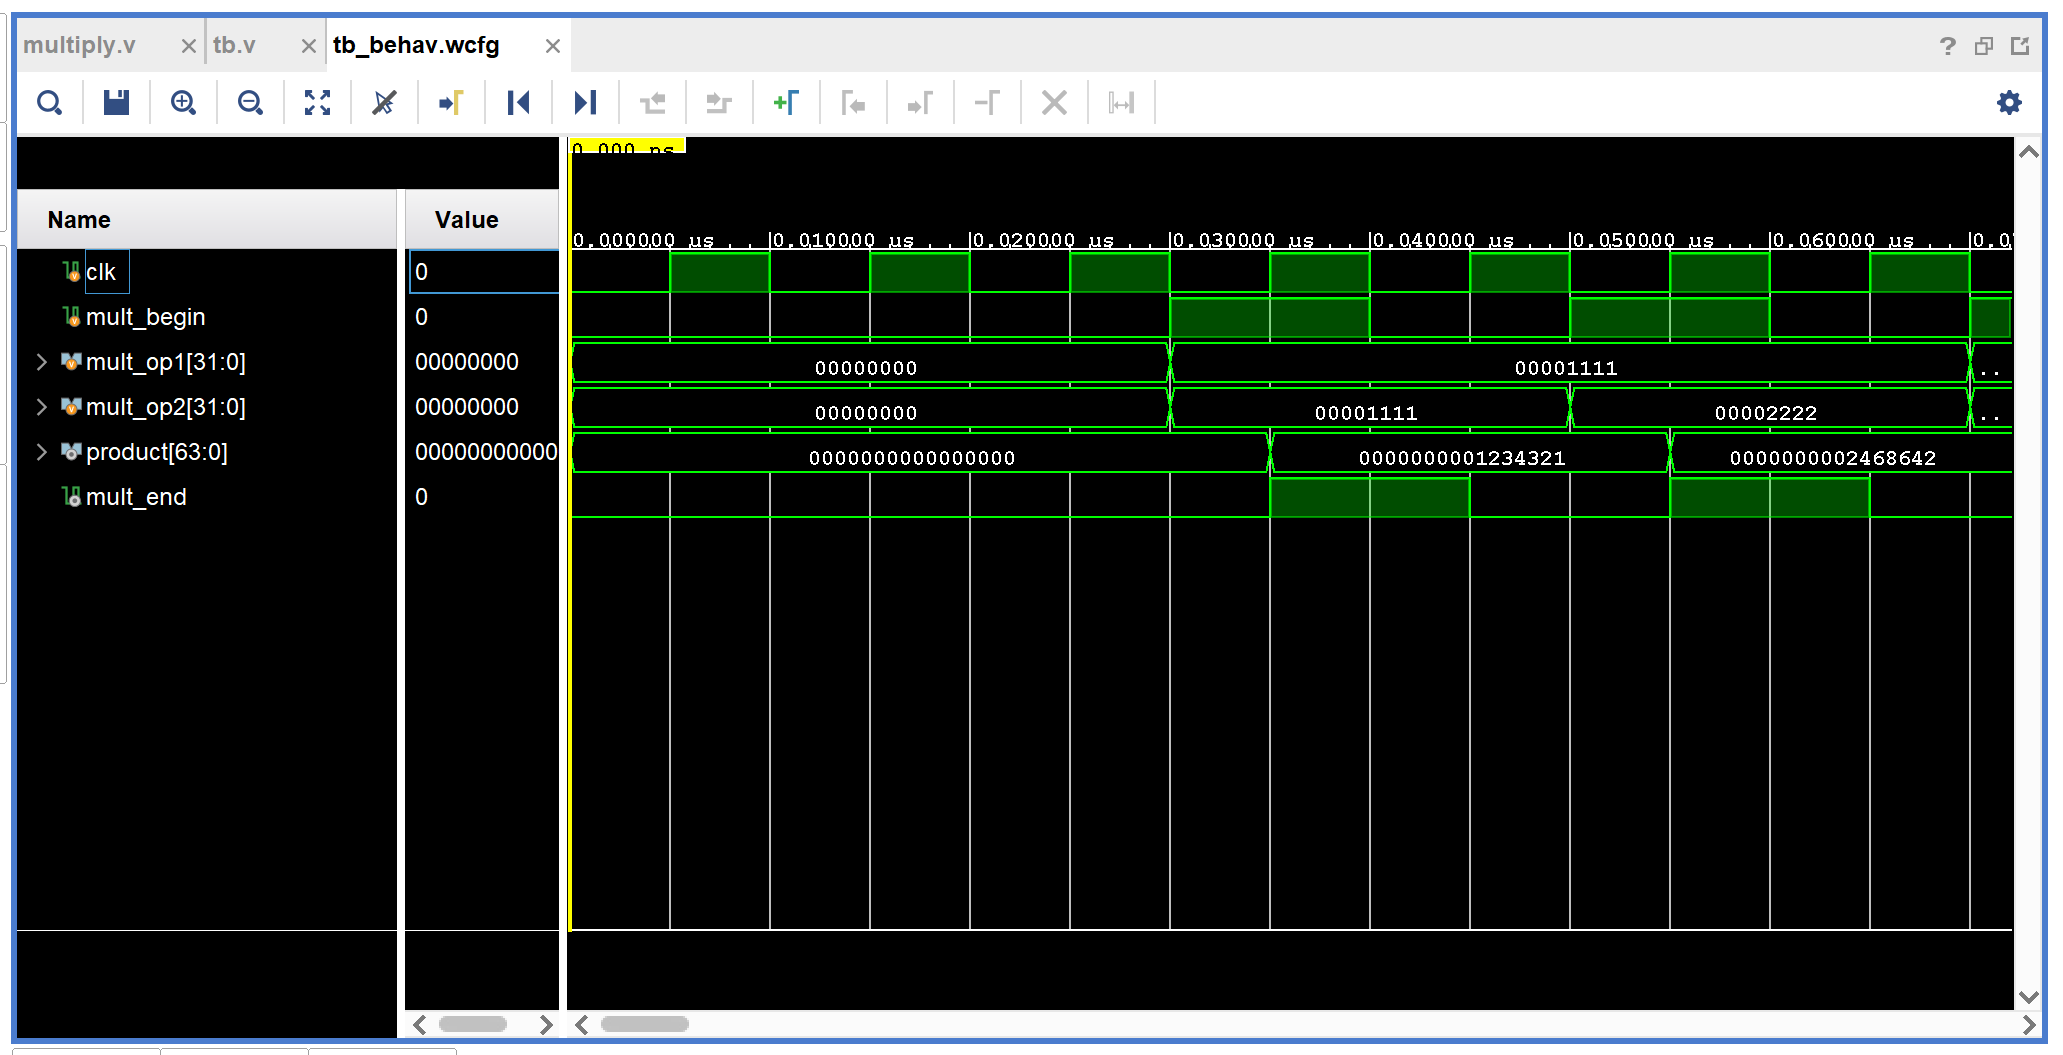
\includegraphics[width=\textwidth]{waveform.png}
\end{figure}

\newpage
\subsection{综合与实现}
\begin{figure}[h!]
    \centering
    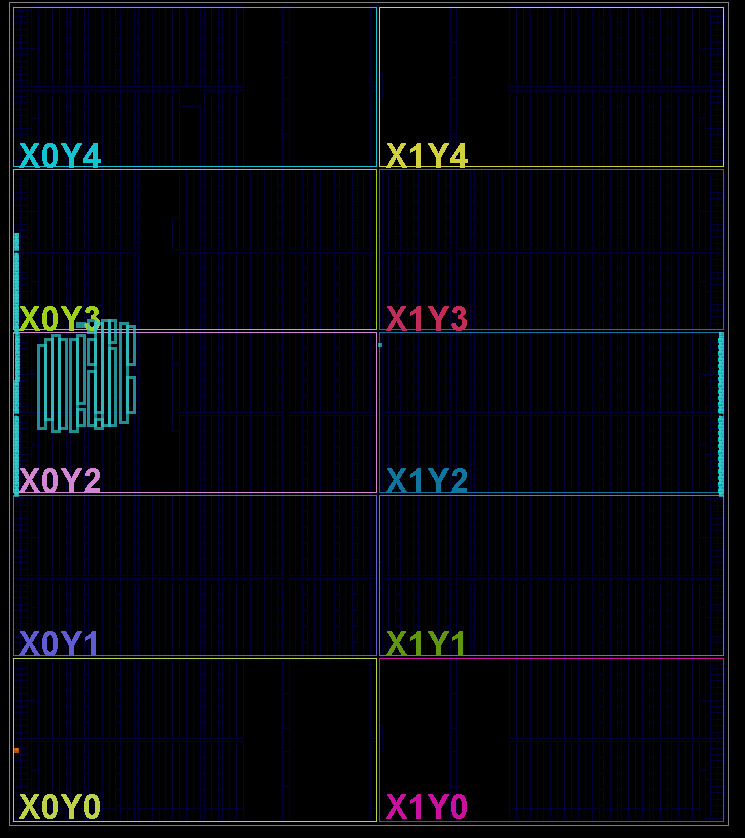
\includegraphics[width=\textwidth]{implement.png}
    \caption{乘法器实现}
    \label{fig:implementation}
\end{figure}

\newpage
\subsection{上板验证}
[CASE 10] PASS: a=12153524(303379748), b=c0895e81(-1064739199),

product=fb8466bd5676ff24(-323020309878341852), cycles=1
\begin{figure}[H]
    \centering
    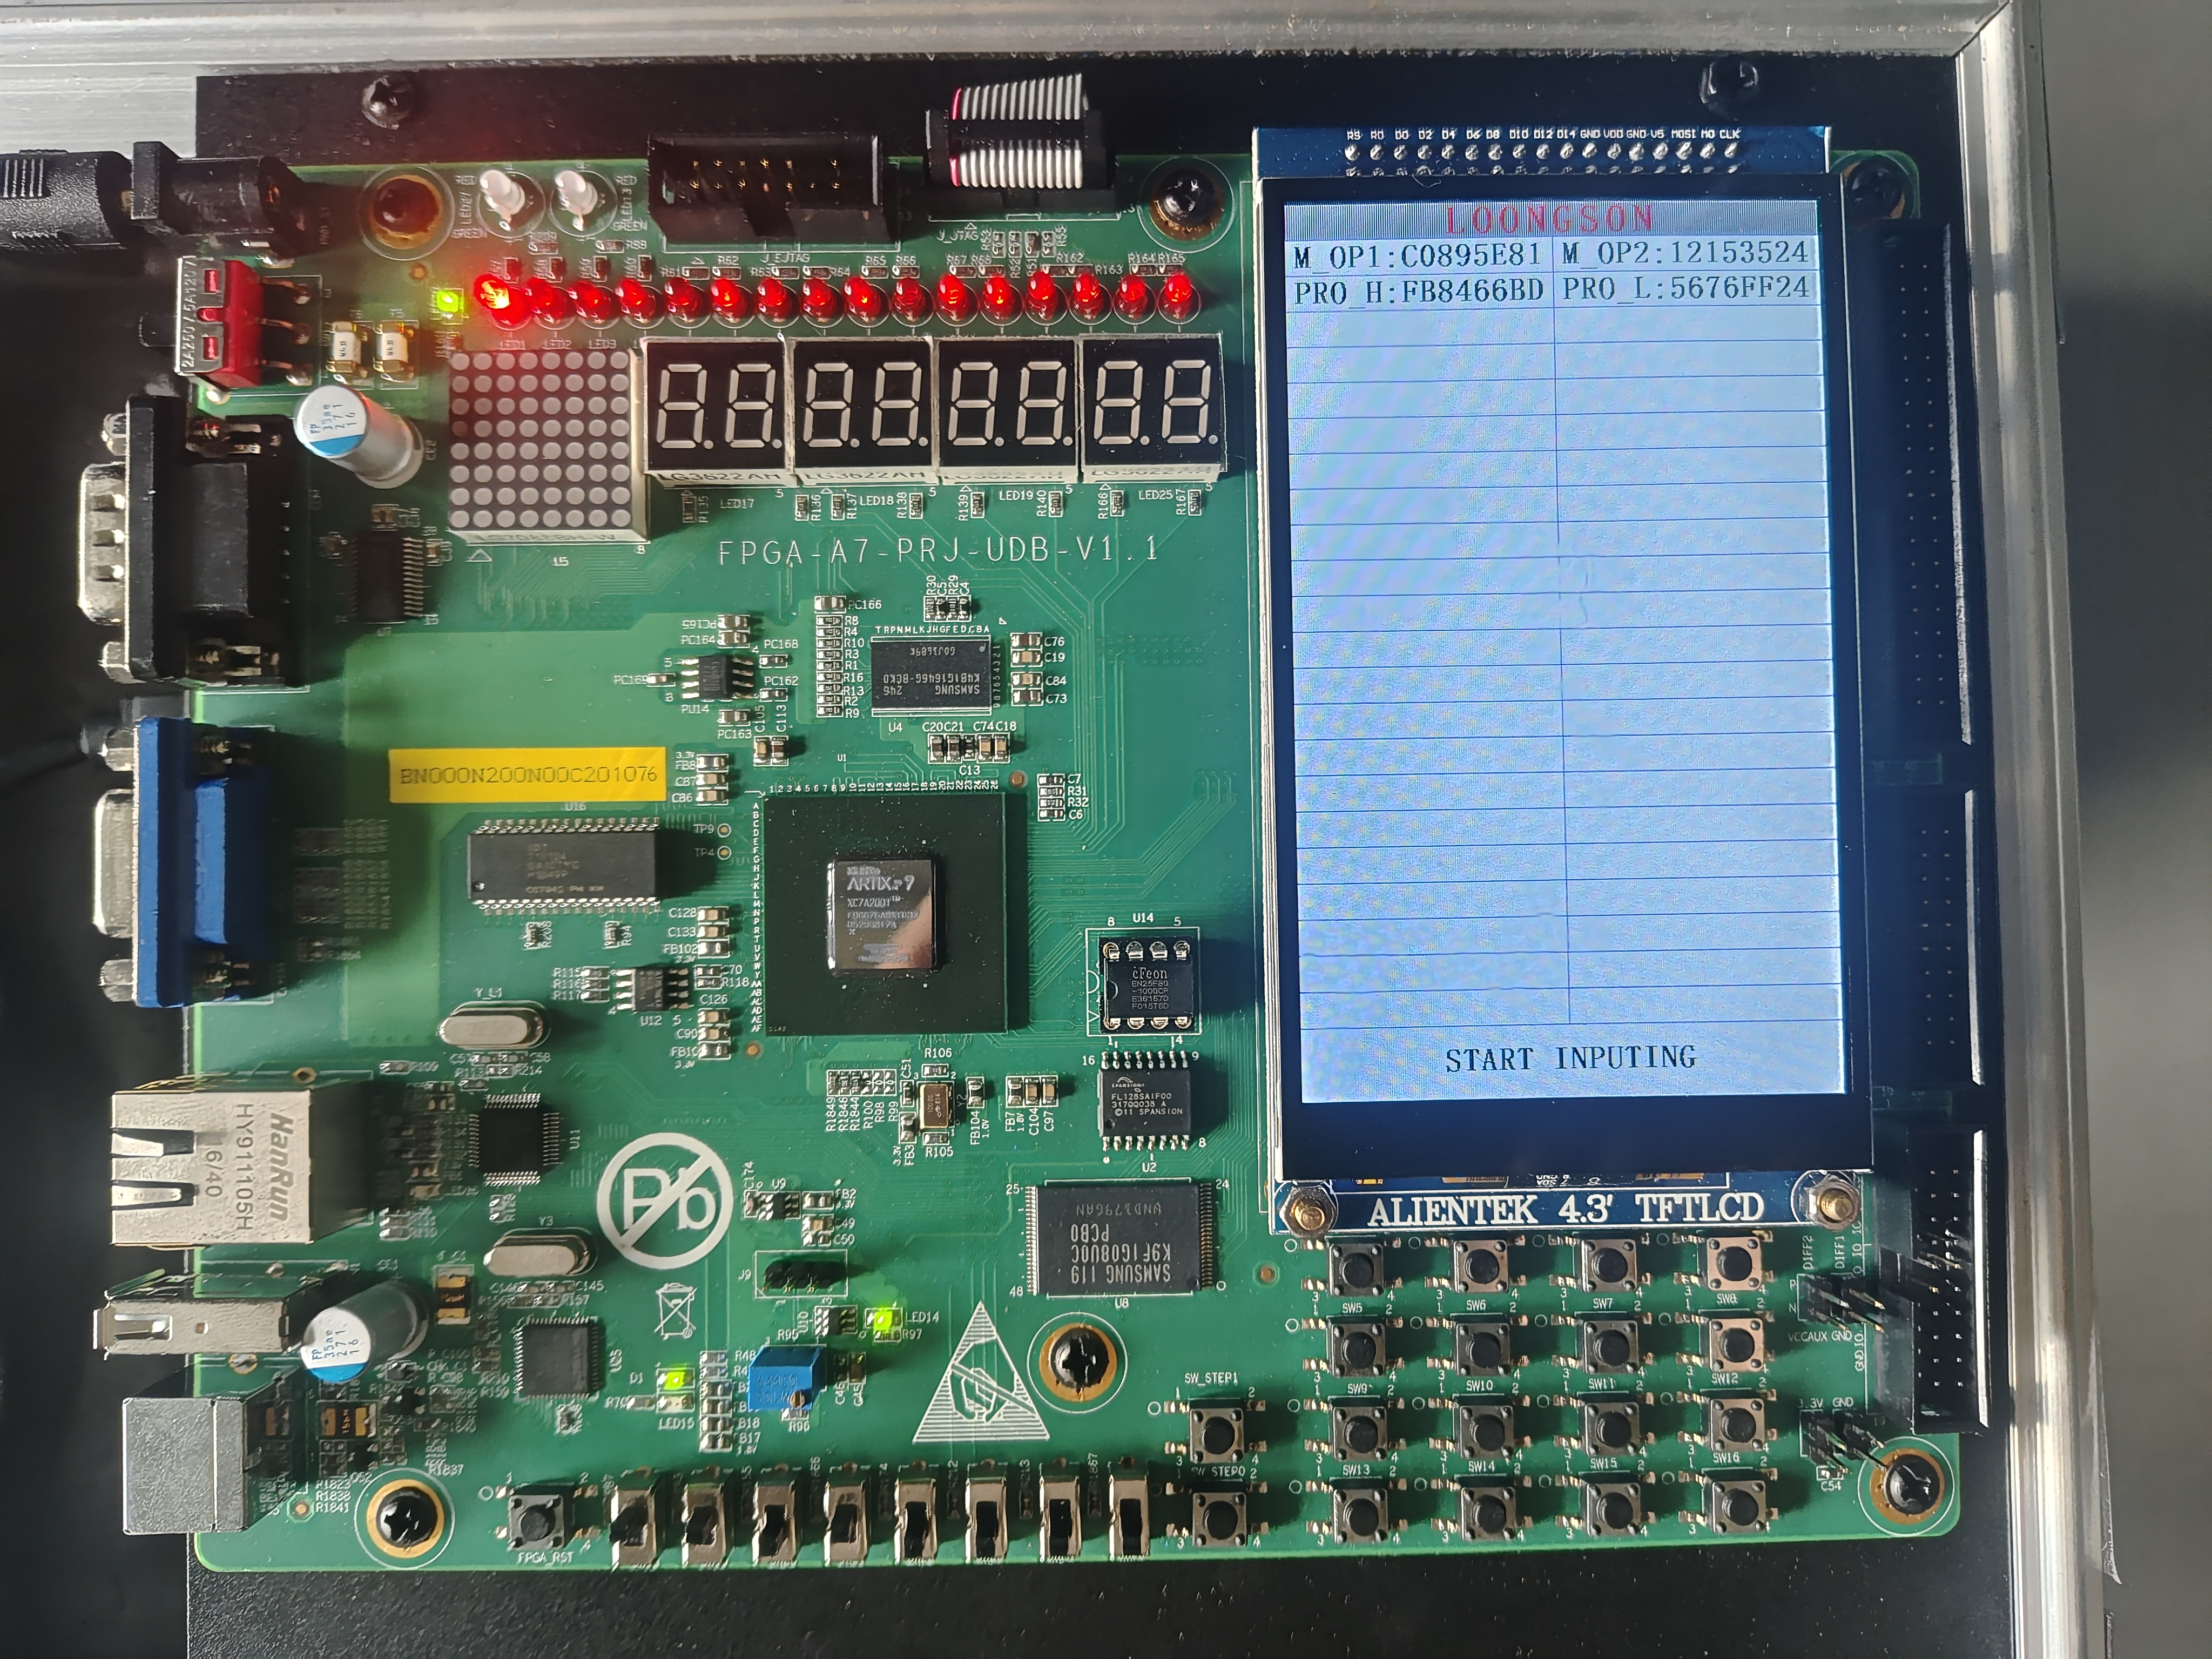
\includegraphics[width=\textwidth]{onboard.jpg}
    \caption{实验箱上板验证}
    \label{fig:board_photo}
\end{figure}

\section{实验收获}
\begin{itemize}
    \item 理解了串行移位乘法器的设计
    \item 学习到Booth编码和Wallace树对乘法器的优化
    \item 直观感受到算术单元设计对硬件利用和设备性能的影响
\end{itemize}

\section{附：源码目录}
\begin{itemize}
\item \verb|lab2/lab2.srcs/sources_1/imports/1012/adder.v|
\item \verb|lab2/lab2.srcs/sources_1/imports/1012/adder_display.v|
\item \verb|lab2/lab2.srcs/sim_1/imports/1012/testbench.v|
\item \verb|lab2/lab2.srcs/constrs_1/imports/1012/multiply.xdc|
\end{itemize}
\end{document}
